\documentclass[12pt,twoside]{book}

\usepackage[paperheight=16cm,paperwidth=12cm,textwidth=10cm]{geometry}
\pagestyle{plain}
\usepackage[utf8]{inputenc}
\usepackage[T1]{fontenc}
\usepackage[portuguese]{babel}
\usepackage{hyphenat}
\usepackage{graphicx}
\usepackage{amsmath}
\usepackage{amssymb}

\title{\vspace{90pt}\textbf{\color{white} A Era da Inteligência Artificial: Transformações e Desafios para o Futuro da Sociedade}}

\date{}
%adicionando imagem na capa 
\usepackage{eso-pic}
\newcommand\BackgroundPic{%
\put(0,0){%
\parbox[b][\paperheight]{\paperwidth}{%
\vfill
\centering
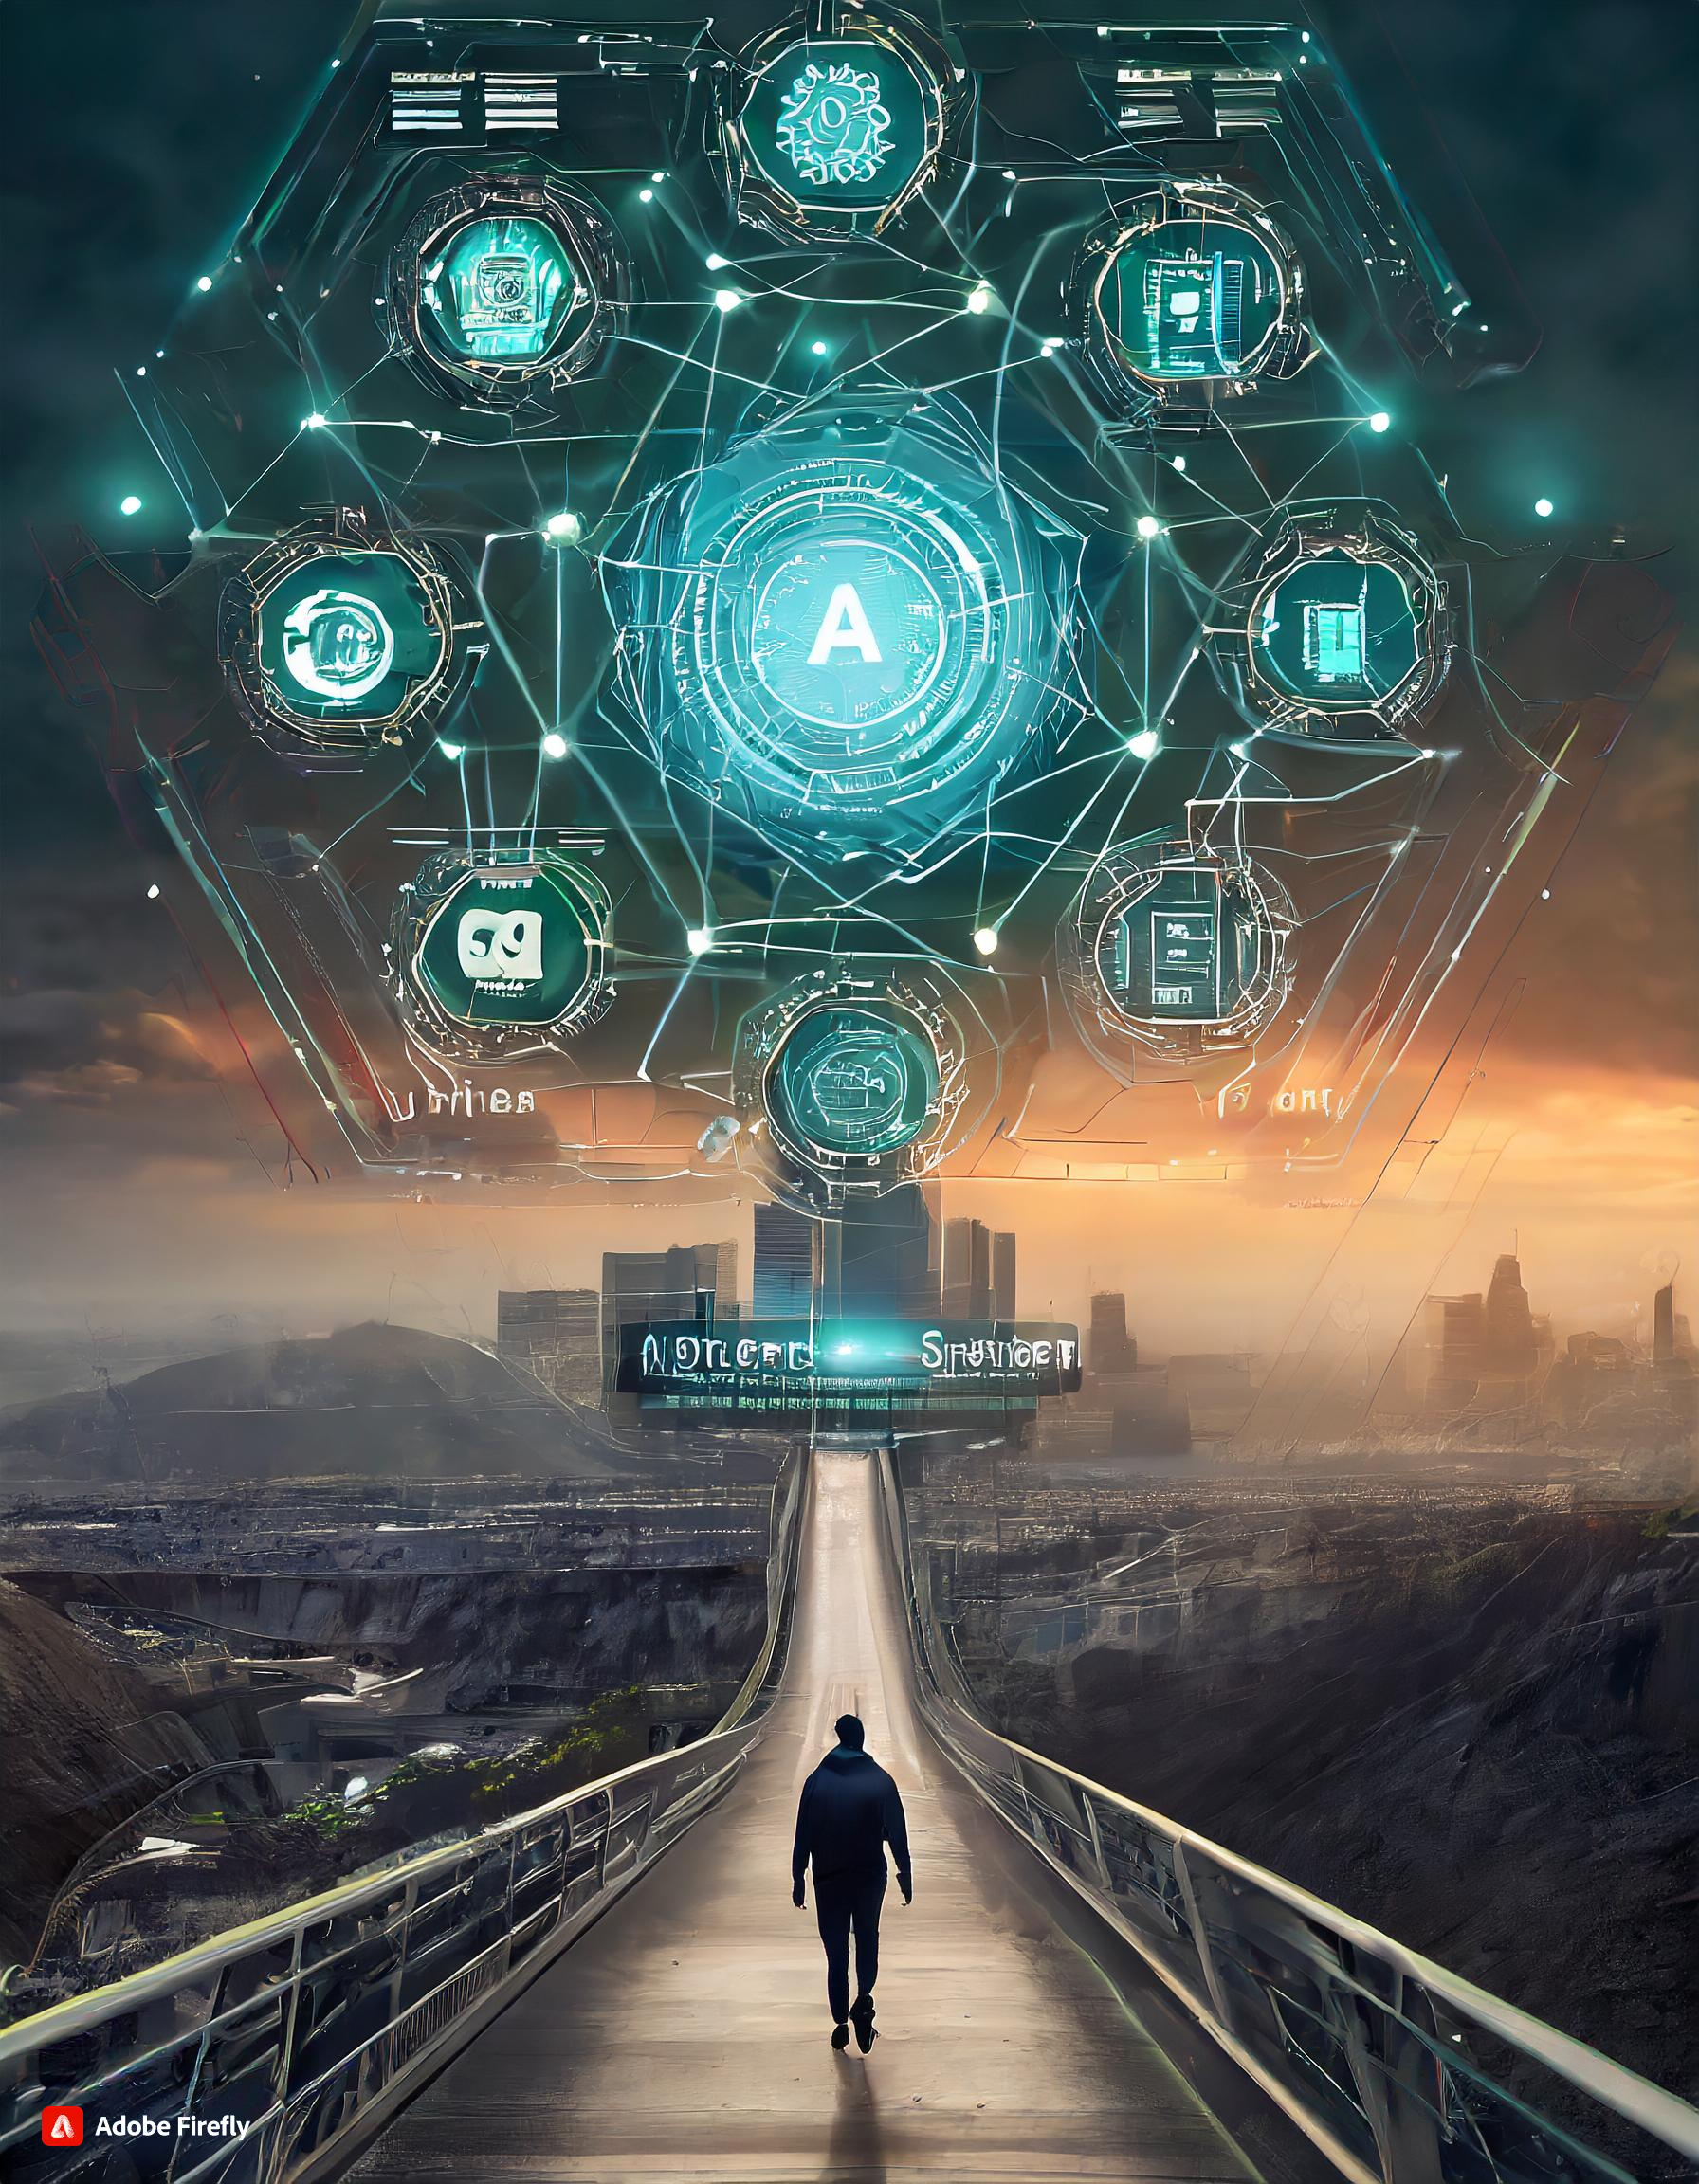
\includegraphics[width=\paperwidth,height=\paperheight,%
keepaspectratio]{capa.jpg}%
\vfill
}}}
\begin{document}
\AddToShipoutPicture*{\BackgroundPic}
\maketitle

\tableofcontents

\chapter{Introdução}

A inteligência artificial (IA) está revolucionando a sociedade em um ritmo acelerado, impulsionando mudanças em diversos setores, desde a saúde e o transporte até a educação e o entretenimento. Essa tecnologia disruptiva tem o potencial de automatizar tarefas repetitivas e complexas, liberando o tempo humano para atividades mais criativas e estratégicas.

No entanto, essa transformação também traz consigo desafios e incertezas. Um dos principais impactos da IA será no mercado de trabalho, com a potencial extinção de diversos cargos tradicionais. Ao mesmo tempo, novas oportunidades surgirão, exigindo habilidades e conhecimentos específicos para acompanhar a demanda por profissionais qualificados na era da IA.

\section{Visão Geral do E-book}

Este e-book se propõe a explorar os impactos da IA na sociedade, com foco em três áreas principais:
\begin{itemize}
    \item Mercado de Trabalho: Análise dos impactos da IA nos diferentes setores da economia, com ênfase nos cargos em risco de extinção e nas novas oportunidades que serão criadas.
    \item Ética da IA: Discussão dos desafios éticos relacionados ao desenvolvimento e utilização da IA, como vieses algorítmicos, perda de privacidade e desigualdade social.
    \item Transformações Sociais: Reflexão sobre as mudanças que a IA trará para a sociedade como um todo, incluindo o impacto na educação, na política, na cultura e nas relações humanas.

\end{itemize}


\section{Objetivos do E-book}

Ao abordar essas temáticas, este e-book busca:
\begin{itemize}
    \item Informar o leitor sobre os impactos da IA na sociedade, de forma clara e objetiva.
    \item Estimular a reflexão crítica sobre os desafios éticos da IA e as medidas necessárias para garantir seu uso responsável.
    \item Preparar o leitor para as mudanças que a IA trará para o mercado de trabalho e para a sociedade como um todo, fornecendo ferramentas para navegar nesse novo cenário.
\end{itemize}

\section{Metodologia}

Para alcançar seus objetivos, este e-book se baseia em:
\begin{itemize}
    \item Pesquisa bibliográfica em livros, artigos científicos e relatórios de instituições renomadas.
    \item Análise de estudos de caso que demonstram os impactos da IA em diferentes setores da sociedade.
    \item Consulta a especialistas em IA para obter diferentes perspectivas sobre o tema.
\end{itemize}

\section{Estrutura do E-book}

O e-book está dividido em cinco capítulos:
\begin{itemize}
    \item Capítulo 1: Introdução à IA e seus impactos na sociedade.
    \item Capítulo 2: Mercado de trabalho: Empregos em risco e novas oportunidades.
    \item Capítulo 3: Ética da IA: Desafios e medidas para um uso responsável.
    \item Capítulo 4: Transformações sociais: O impacto da IA na educação, na política, na cultura e nas relações humanas.
    \item Capítulo 5: Conclusões e perspectivas para o futuro da IA.
\end{itemize}

\section{Público-Alvo}

Este e-book destina-se a um público amplo, incluindo:
\begin{itemize}
    \item Estudantes e profissionais interessados em compreender os impactos da IA na sociedade.
    \item Tomadores de decisão em empresas e governos que precisam formular políticas para o desenvolvimento e uso da IA.
    \item Cidadãos que desejam se preparar para as mudanças que a IA trará para o futuro do trabalho e da sociedade.
\end{itemize}

Esperamos que este e-book seja uma fonte útil de informação e reflexão sobre 
os impactos da IA na sociedade.

\chapter{Mercado de Trabalho: Empregos em Risco e Novas Oportunidades na Era da IA}


A inteligência artificial (IA) está transformando o mercado de trabalho em um ritmo acelerado. A automação de tarefas repetitivas e complexas ameaça a existência de diversos cargos tradicionais, enquanto novas oportunidades surgem em áreas que exigem criatividade, adaptabilidade e habilidades digitais.

\section{Empregos em Risco}

Os setores mais impactados pela automação incluem:
\begin{itemize}
    \item Produção: A automação de fábricas e linhas de produção pode eliminar milhões de empregos, principalmente aqueles que exigem pouca qualificação e repetitividade.
    \item Administração: A digitalização de processos administrativos e a automatização de tarefas repetitivas podem levar à extinção de cargos como digitadores, arquivistas e caixa de banco.
    \item Transporte: O desenvolvimento de carros autônomos pode levar ao fim da profissão de motorista de táxi, ônibus e caminhão.
    \item Telemarketing: A automação de chatbots e sistemas de atendimento ao cliente pode eliminar a necessidade de operadores de telemarketing.

\end{itemize}


\section{Novas Oportunidades}

Ao mesmo tempo que a IA elimina alguns cargos, ela também cria novas oportunidades em áreas como:
\begin{itemize}
    \item Desenvolvimento de IA: Profissionais especializados em programação, ciência de dados e engenharia de software serão altamente requisitados para o desenvolvimento e aprimoramento de sistemas de IA.
    \item Análise de dados: A grande quantidade de dados gerados pela IA demandará profissionais qualificados para interpretá-los e transformá-los em insights estratégicos para as empresas.
    \item Cuidados com a saúde: A IA será utilizada para auxiliar no diagnóstico de doenças, desenvolvimento de medicamentos personalizados e até mesmo na realização de cirurgias robóticas.
    \item Educação: A IA será utilizada para personalizar o aprendizado, criar plataformas de ensino online e desenvolver ferramentas de avaliação automatizada.
\end{itemize}

\section{Habilidades Necessárias para o Futuro do Trabalho}

Para se destacar no mercado de trabalho da era da IA, será necessário desenvolver habilidades como:
\begin{itemize}
    \item Criatividade: A IA não é capaz de substituir a criatividade humana, que será essencial para a resolução de problemas complexos e a geração de novas ideias.
    \item Adaptabilidade: A capacidade de se adaptar a novas tecnologias e métodos de trabalho será fundamental para acompanhar as mudanças constantes do mercado.
    \item Pensamento crítico: A capacidade de analisar informações, identificar vieses e tomar decisões embasadas será crucial para o sucesso profissional.
    \item Habilidades digitais: O domínio de ferramentas digitais, como programação, análise de dados e comunicação online, será essencial para a maioria das carreiras.
\end{itemize}

\section{Medidas para Mitigar os Impactos Negativos da IA}

Para minimizar os impactos negativos da IA no mercado de trabalho, é necessário:
\begin{itemize}
    \item Investir em educação e treinamento: Preparar a força de trabalho para as novas demandas do mercado, com foco em habilidades como criatividade, adaptabilidade e pensamento crítico.
    \item Criar programas de requalificação: Auxiliar os trabalhadores que perderam seus empregos para a automação a se adaptarem às novas oportunidades.
    \item Implementar políticas de renda básica: Garantir um nível mínimo de renda para todos os cidadãos, independentemente de sua situação profissional.
\end{itemize}

A IA está transformando o mercado de trabalho de forma profunda e irreversível. É fundamental que os governos, empresas e indivíduos se preparem para essa transformação, investindo em educação, treinamento e políticas públicas que minimizem os impactos negativos e maximizem os benefícios da IA para a sociedade.

\chapter{Ética da IA: Desafios e Medidas para um Uso Responsável na Era da Informação}

A inteligência artificial (IA) abre um mundo de possibilidades para a sociedade, mas também levanta preocupações éticas que exigem atenção e medidas proativas. É crucial que o desenvolvimento e a utilização da IA sejam guiados por princípios éticos sólidos para garantir que seus benefícios sejam distribuídos de forma justa e que seus riscos sejam minimizados.

\section{Desafios Éticos da IA}

Os principais desafios éticos da IA incluem:
\begin{itemize}
    \item Vieses algorítmicos: Os algoritmos de IA podem perpetuar vieses existentes na sociedade, como discriminação racial, de gênero e socioeconômica. É fundamental que os desenvolvedores de IA estejam conscientes desses vieses e adotem medidas para mitigá-los.
    \item Perda de privacidade: A coleta massiva de dados pessoais para o treinamento de algoritmos de IA levanta preocupações sobre privacidade e segurança. É necessário garantir que esses dados sejam coletados e utilizados de forma ética e responsável.
    \item Desigualdade social: A IA pode exacerbar a desigualdade social, concentrando os benefícios nas mãos de uma minoria e deixando para trás os grupos mais vulneráveis. É fundamental que os governos e empresas tomem medidas para garantir que a IA seja utilizada de forma inclusiva e equitativa.
    \item Transparência algorítmica: A falta de clareza sobre como os algoritmos de IA funcionam pode levar à desconfiança e à falta de controle sobre as decisões tomadas por esses sistemas. É fundamental que os algoritmos sejam transparentes e explicáveis.
    \item Autonomia e responsabilidade: A crescente autonomia dos sistemas de IA levanta questões sobre responsabilidade em caso de erros ou falhas. É necessário estabelecer mecanismos para garantir que os agentes de IA sejam responsáveis por suas ações.
\end{itemize}

\section{Medidas para um Uso Responsável da IA}

Para garantir um uso ético da IA, é necessário:
\begin{itemize}
    \item Criar leis e normas que regulem o desenvolvimento e a utilização da IA.
    \item Estabelecer princípios éticos para o desenvolvimento e uso da IA.
    \item Promover a transparência e a explicabilidade dos algoritmos de IA.
    \item Investir em educação e treinamento para a população sobre a IA.
    \item Criar mecanismos de participação pública no processo de desenvolvimento da IA.
    \item Promover a colaboração entre governos, empresas e sociedade civil para garantir um desenvolvimento ético da IA.
\end{itemize}

\subsection{Exemplos de Iniciativas Éticas em IA}

Diversas iniciativas estão sendo tomadas para promover o uso ético da IA, como:
\begin{itemize}
    \item A "Carta de Ética da Inteligência Artificial" da Comissão Europeia, que define princípios éticos para o desenvolvimento e uso da IA na Europa.
    \item Os "Princípios de Toronto para a IA", que estabelecem diretrizes éticas para o desenvolvimento e uso da IA.
    \item O "Instituto de Inteligência Artificial da Universidade de Stanford", que pesquisa e promove o desenvolvimento ético da IA.
\end{itemize}

A IA é uma ferramenta poderosa que pode ser utilizada para o bem ou para o mal. É fundamental que a sociedade se mobilize para garantir que a IA seja utilizada de forma ética e responsável, para que seus benefícios sejam distribuídos de forma justa e que seus riscos sejam minimizados. Através de um diálogo aberto e da colaboração entre diferentes setores da sociedade, podemos construir um futuro onde a IA seja uma força para o bem de todos.

\chapter{Transformações Sociais: O Impacto da IA na Educação, na Política, na Cultura e nas Relações Humanas na Era da Informação}

A inteligência artificial (IA) está revolucionando a sociedade em um ritmo acelerado, e seus impactos se estendem para além do mercado de trabalho. A IA tem o potencial de transformar áreas como a educação, a política, a cultura e as relações humanas, trazendo consigo oportunidades e desafios que precisam ser cuidadosamente analisados.

\section{Educação}

A IA pode revolucionar a educação, personalizando o aprendizado para cada aluno, criando plataformas de ensino online e desenvolvendo ferramentas de avaliação automatizada. Algumas das principais mudanças que podemos esperar na educação incluem:
\begin{itemize}
    \item Aprendizado personalizado: A IA pode analisar o estilo de aprendizado de cada aluno e adaptar os conteúdos e atividades para atender às suas necessidades individuais.
    \item Ensino online: A IA pode ser utilizada para criar plataformas de ensino online que oferecem cursos e materiais didáticos de alta qualidade para qualquer pessoa, em qualquer lugar do mundo.
    \item Avaliação automatizada: A IA pode ser utilizada para desenvolver ferramentas que avaliam automaticamente o desempenho dos alunos, fornecendo feedback instantâneo e personalizado.
\end{itemize}

\section{Política}

A IA pode ser utilizada para melhorar a eficiência da gestão pública, aumentar a transparência e a participação dos cidadãos na tomada de decisões e fortalecer a democracia. No entanto, também existem preocupações sobre o potencial da IA para ser utilizada para manipular a opinião pública e controlar a população. Algumas das principais mudanças que podemos esperar na política incluem:
\begin{itemize}
    \item Gestão pública mais eficiente: A IA pode ser utilizada para automatizar tarefas repetitivas, reduzir custos e melhorar a qualidade dos serviços públicos.
    \item Maior transparência: A IA pode ser utilizada para tornar os dados públicos mais acessíveis e transparentes, permitindo que os cidadãos acompanhem as ações do governo.
    \item Participação cidadã: A IA pode ser utilizada para criar plataformas que facilitam a participação dos cidadãos na tomada de decisões políticas.
\end{itemize}

\section{Cultura}

A IA pode ser utilizada para criar novas formas de arte, música e literatura, democratizar o acesso à cultura e promover a inclusão social. No entanto, também existem preocupações sobre o potencial da IA para ser utilizada para criar conteúdo falso e manipular as emoções das pessoas. Algumas das principais mudanças que podemos esperar na cultura incluem:
\begin{itemize}
    \item Novas formas de arte: A IA pode ser utilizada para criar novas formas de arte, como pinturas, músicas e poemas gerados por algoritmos.
    \item Democratização da cultura: A IA pode ser utilizada para tornar a cultura mais acessível a todos, por exemplo, através da tradução automática de obras literárias e da criação de plataformas de streaming de conteúdo cultural.
    \item Inclusão social: A IA pode ser utilizada para promover a inclusão social, por exemplo, através da criação de ferramentas de comunicação para pessoas com deficiência.
\end{itemize}

\section{Relações Humanas}

A IA pode ter um impacto significativo nas relações humanas, tanto em ambientes profissionais quanto pessoais. Algumas das principais mudanças que podemos esperar nas relações humanas incluem:
\begin{itemize}
    \item Novas formas de trabalho: A IA pode levar à criação de novos tipos de trabalho que exigem habilidades em áreas como programação, análise de dados e desenvolvimento de IA.
    \item Mudanças na comunicação: A IA pode mudar a forma como nos comunicamos, por exemplo, através do uso de chatbots e assistentes virtuais.
    \item Novas formas de relacionamento: A IA pode criar novas formas de relacionamento, por exemplo, através de plataformas de namoro online e jogos online.
\end{itemize}

A IA é uma tecnologia poderosa que tem o potencial de transformar a sociedade de forma profunda e irreversível. É fundamental que a sociedade se prepare para essa transformação, discutindo os desafios e oportunidades que a IA apresenta e buscando soluções para garantir que seus benefícios sejam distribuídos de forma justa e que seus riscos sejam minimizados. Através de um diálogo aberto e da colaboração entre diferentes setores da sociedade, podemos construir um futuro onde a IA seja uma força para o bem de todos.

\chapter{Conclusões e Perspectivas para o Futuro da IA na Era da Informação}

A inteligência artificial (IA) está revolucionando a sociedade em um ritmo acelerado, impactando o mercado de trabalho, a educação, a política, a cultura e as relações humanas. As mudanças trazidas pela IA são complexas e exigem uma análise cuidadosa para garantir que seus benefícios sejam distribuídos de forma justa e que seus riscos sejam minimizados.

Com base nos capítulos anteriores, podemos concluir que a IA apresenta um enorme potencial para a sociedade, mas também traz consigo desafios e incertezas. Para garantir que a IA seja uma força para o bem, é fundamental:

Investir em pesquisa e desenvolvimento de IA responsável: Assegurar que a IA seja desenvolvida e utilizada de forma ética e responsável, com foco no bem-estar social.

Promover a educação e a capacitação da população em IA: Preparar a sociedade para as mudanças trazidas pela IA, dotando os indivíduos das habilidades necessárias para navegar nesse novo cenário.

Criar políticas públicas que regulem o desenvolvimento e a utilização da IA: Garantir que a IA seja utilizada de forma justa e equitativa, protegendo os direitos dos indivíduos e da sociedade.

Promover o diálogo entre os diferentes setores da sociedade: Buscar soluções para os desafios da IA através da colaboração entre governos, empresas, academia e sociedade civil.

\section{Perspectivas para o Futuro da IA}

O futuro da IA é incerto, mas algumas tendências podem ser observadas:
\begin{itemize}
    \item A IA se tornará cada vez mais pervasiva: A IA estará presente em todos os aspectos da vida, desde o trabalho até o lazer.
    \item A IA se tornará mais autônoma: Os sistemas de IA serão capazes de tomar decisões complexas sem a necessidade de intervenção humana.
    \item A IA se tornará mais interligada: Os sistemas de IA serão capazes de se comunicar e colaborar entre si, criando uma "rede de inteligência".
\end{itemize}

Essas tendências trazem consigo grandes desafios, mas também abrem novas oportunidades para a sociedade. É fundamental que nos preparemos para esse futuro, buscando soluções para os desafios da IA e aproveitando suas oportunidades para construir um mundo melhor para todos.

\end{document}
